%!TEX root = ./intern_report.tex

\newpage
\subsection{Building Wallie: A Hardware Platform for Data Collection and Deployment}

To collect data, I sketched a small camera rig to hold three Intel Realsense cameras, each facing center, left and right at 30 degree angles from center. Samith Ashan, my coworker helped us by designing it in solidworks. With the help of other CSIRO members, we 3D-printed the camera rig. 

\begin{figure}[H]
    \centering
    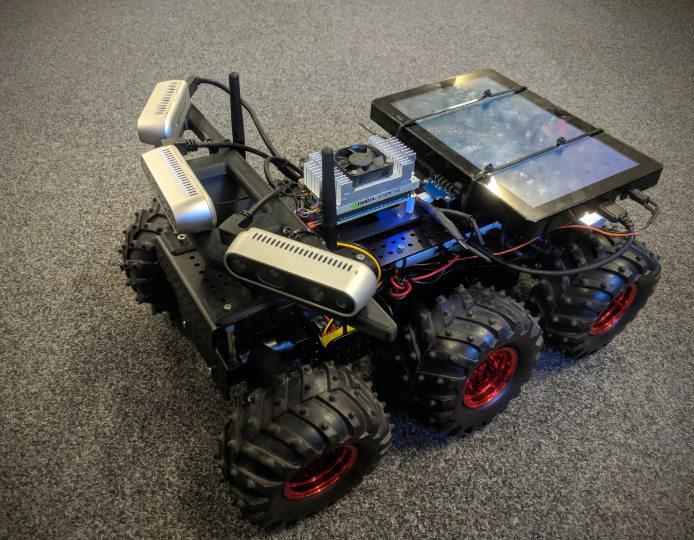
\includegraphics
        [width=10cm]
        {figures/wallie.PNG}
    \caption{Wallie: The Robot \label{Fig:wallie}}\vspace{-4mm}
\end{figure}

\begin{figure}[H]
    \centering
    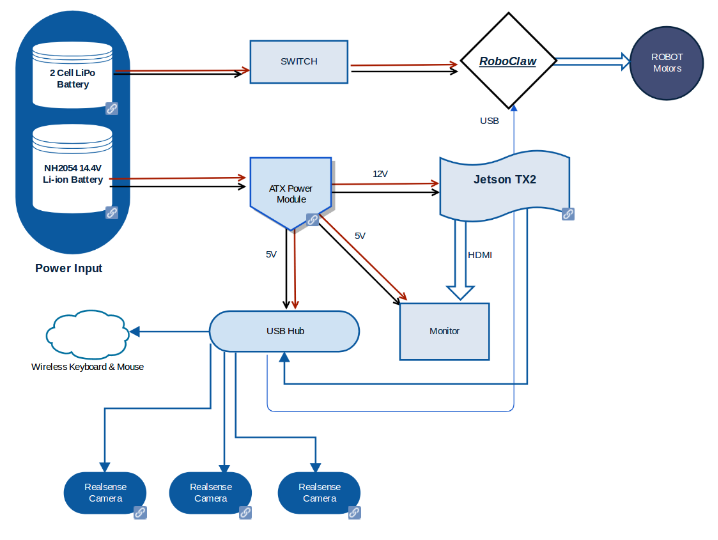
\includegraphics
        [width=10cm]
        {figures/wallie_hardware.PNG}
    \caption{Wallie: Hardware Hierarchy }\vspace{-4mm}
\end{figure}


\subsubsection*{NVIDIA Jetson TX2}

\begin{figure}[H]
    \centering
    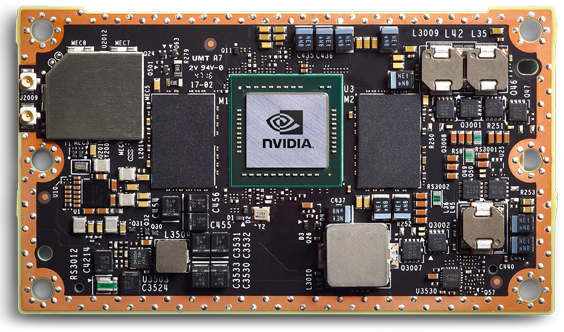
\includegraphics
        [width=8cm]
        {figures/jetson.png}
    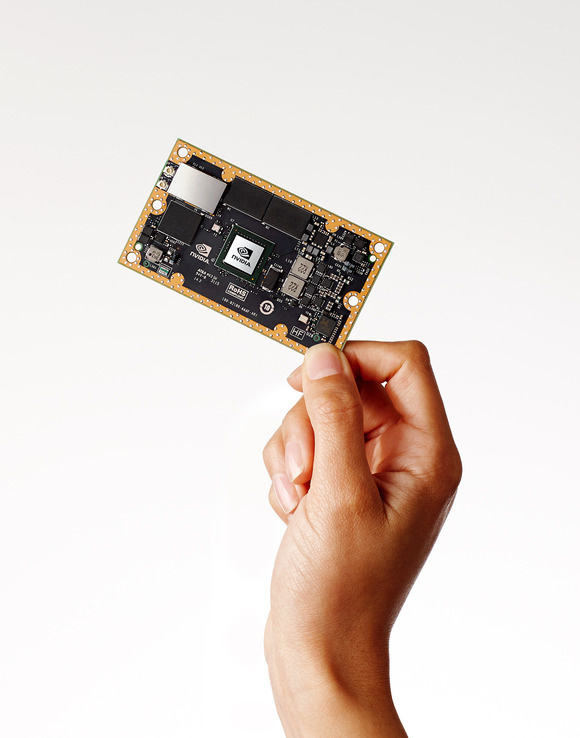
\includegraphics
        [height=5cm]
        {figures/jetson_scale.jpg}
    \caption{NVIDIA Jetson TX2 }\vspace{-4mm}
\end{figure}



\subsubsection*{Intel Realsense Depth Camera D435}

\begin{figure}[H]
    \centering
    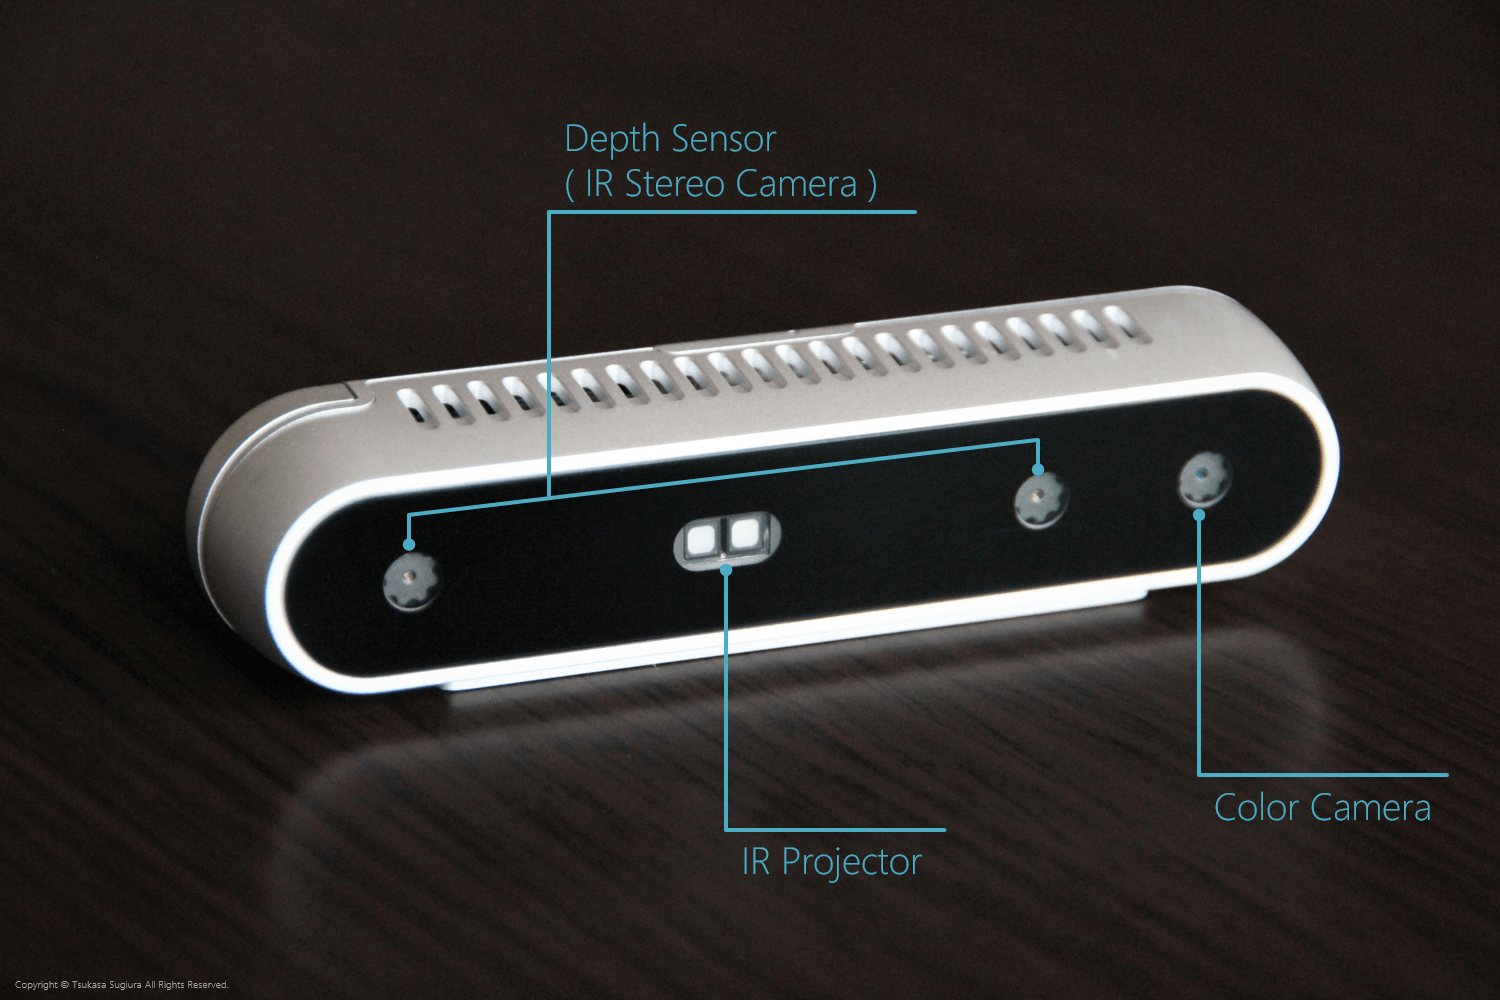
\includegraphics
        [width=12cm]
        {figures/realsense.png}
    \caption{Intel Realsense D435}\vspace{-4mm}
\end{figure}

\subsubsection*{Roboclaw Motor Controller}

\begin{figure}
    \centering
    \begin{minipage}{.5\textwidth}
        \centering
        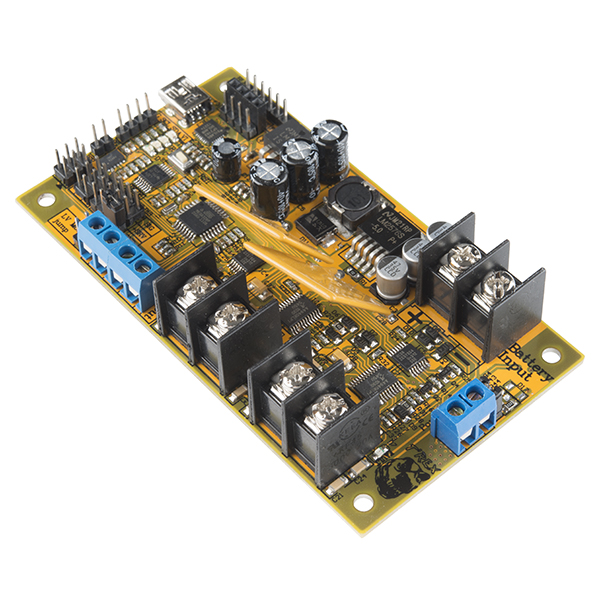
\includegraphics[width=\linewidth]{figures/trex.jpg}
        \captionof{figure}{TREX Motor Controller}
        \label{fig:test1}
    \end{minipage}%
    \begin{minipage}{.5\textwidth}
        \centering
        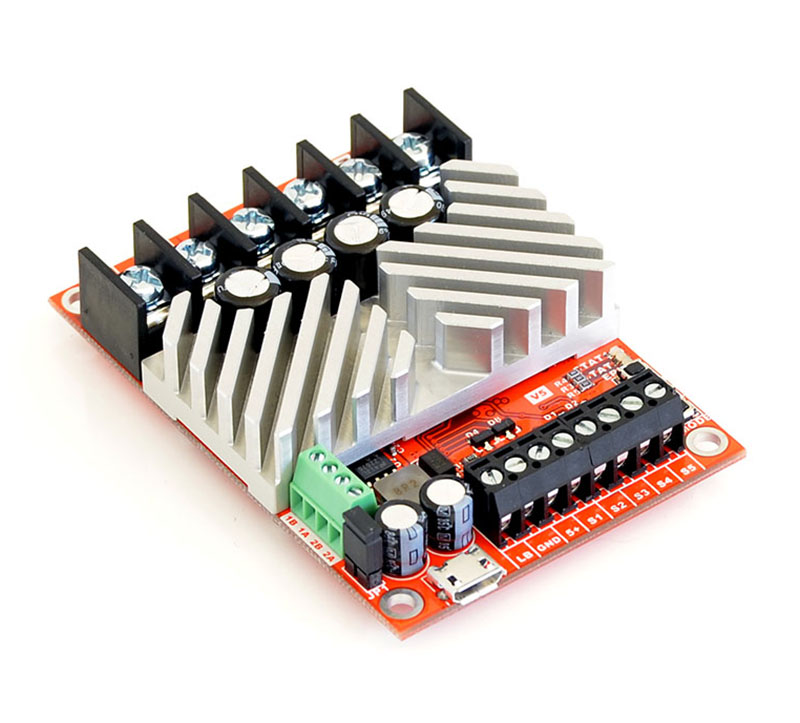
\includegraphics[width=\linewidth]{figures/roboclaw.jpg}
        \captionof{figure}{Roboclaw Motor Controller}
        \label{fig:test1}
    \end{minipage}
\end{figure}



\subsubsection*{Problems Faced and Solutions}